\section{Stream Benchmark}

For a long time we have witness how CPUs are being getting faster much more quickly than the computer's memory sub-system and, as a consequence, more and more programs are being limited in performance by the memory bandwidth of the system, rather than by the computational performance of the CPU \cite{McCalpin2007}.

It is, therefore, particularly important to know the memory bandwidth of the system you are working with. The STREAM benchmark\cite{McCalpin2007} is a suite of four (Copy, Scale, Add and Triad) simple tests that measures sustainable memory bandwidth (in MB/s) and the corresponding computation rate for simple vector kernels. In general, it is used to measure the evolution of the memory bandwidth of shared memory systems as more computing component are included in the test. Traditionally, the test has been implemented using OpenMP and the computing component are usually referred as threads.

In order to study the capabilities of MPI$_{sm}$ as viable alternative to OpenMP in the context of the shared memory programing model, we considered that the first step is to study the sustainable memory bandwidth achievable using MPI$_{sm}$ and compare it to its OpenMP counterpart.


To achieve this objective, we developed an MPI$_{sm}$ version of the stream test. The stream program that can be downloaded from its web site (http://www.cs.virginia.edu/stream/) already is annotated with directives (\textbf{\#pragma}) to make it a correct OpenMP program. Both programs were run, using various compilers and MPI implementations. Results and lessons learned follow.


Figure \ref{fig:TriadTestBefore} presents results obtained on one system (\textbf{stout}) for the Triad test of the stream suite; results of the other tests (Copy, Scale and Add) are similar. The left plot (a) shows the actual bandwidth achieved while the right plot (b) show the MPI$_{sm}$ to OpenMP ratio obtained.


 

\begin{figure} [h!]
    \centering
    \captionsetup{justification=centering, singlelinecheck=false}
    \begin{subfigure}{.6\textwidth}
      \hspace*{-1.5cm} 
      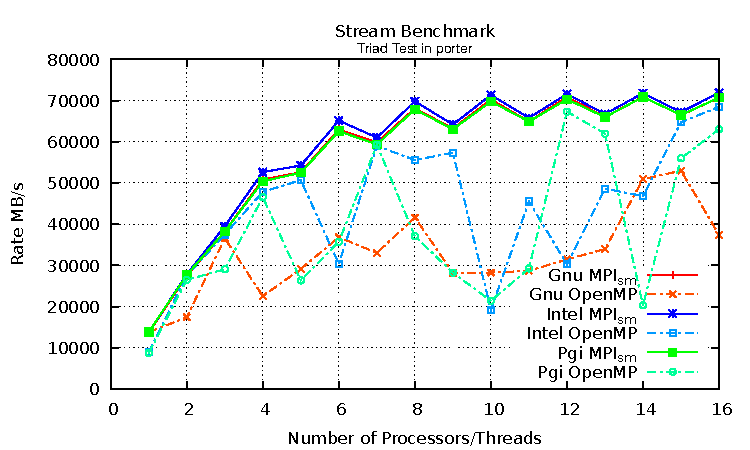
\includegraphics[width=0.95\linewidth]{Plots/streamBenchmark/porter-TriadBefore.pdf}
      \caption[]{Bandwidth per number of processes/threads.}
      \label{fig:TriadBefore}
    \end{subfigure}%
    \begin{subfigure}{.6\textwidth}
      \hspace*{-1.5cm} 
      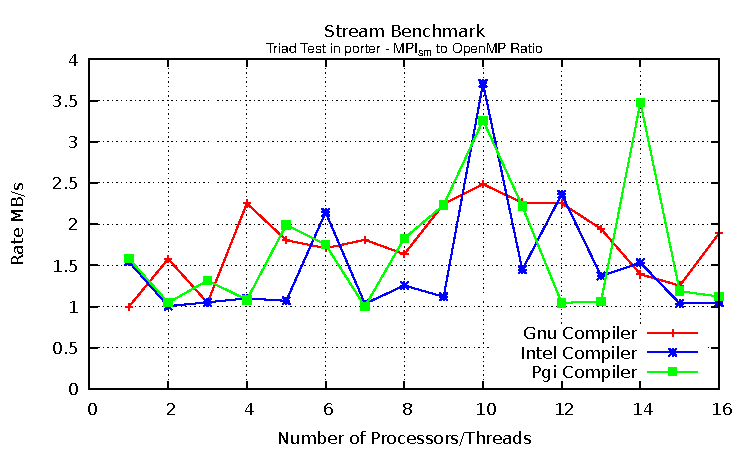
\includegraphics[width=0.95\linewidth]{Plots/streamBenchmark/porter-TriadRatioBefore.pdf}
      \caption{Ratio MPI$_{sm}$ to OpenMP.}
      \label{fig:TriadRatioBefore}
    \end{subfigure}
    \caption{Triad test. No binding policy for OpenMP}
\label{fig:TriadTestBefore}
\end{figure}


Figure \ref{fig:TriadTestBefore}(a) the segmented lines correspond to OpenMP while the continuous lines represent MPI$_{sm}$. Notice the extremely irregular behavior shown by all the OpenMP cases. Exploring the causes of such behavior lead us to our first lesson: \textbf{thread placement}. The lack of a \emph{by-default} thread affinity control policy of all the compilers used in the study results the erratic behavior shown in the figure, because the threads are allow to be moved, by the OS, not only to a different core but also to a different socket.

The OpenMP version 4.0 specification introduces a standard way to control thread affinity, allowing for the first time a standard way to have fine grain control over the affinity policy.  It introduced two new concepts to the language: binding policy and place partition.

The binding policy determines if the threads will be bound and how they will be distributed, while the place partition is the set of places to which threads can be bound. One simple way of control the binding policy is by setting the \textbf{OMP\_PROC\_BIND} environment variable. Similarly, a way of control the place partition is by setting the \textbf{OMP\_PLACES} environment variable. 

In our case, we find convenient to set 

\begin{itemize} 

\item \textbf{OMP\_PROC\_BIND}=spread 

\item \textbf{OMP\_PLACES}=sockets

\end{itemize}

meaning that the threads will be bound and distributed (or spread) among the sockets. More details about the values allowed for these enviromantal variables can be found in the OpenMP API specification.


\begin{figure} [h!]
    \centering
    \captionsetup{justification=centering, singlelinecheck=false}
    \begin{subfigure}{.6\textwidth}
      \hspace*{-1.5cm} 
      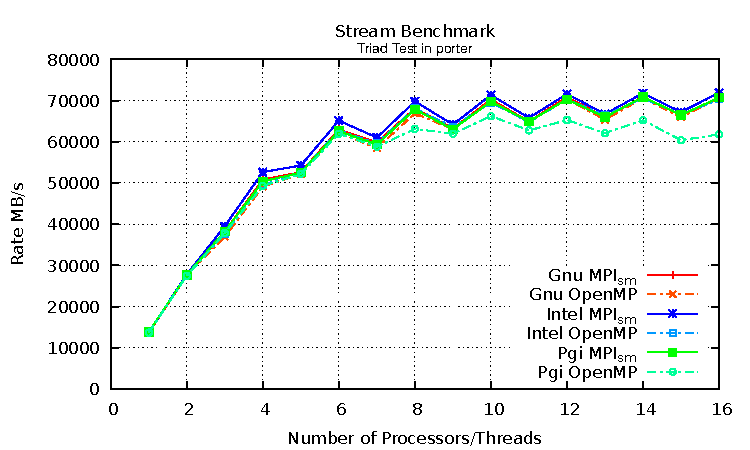
\includegraphics[width=0.95\linewidth]{Plots/streamBenchmark/porter-Triad.pdf}
      \caption[]{Ratio MPI$_{sm}$ to OpenMP.}
      \label{fig:Triad}
    \end{subfigure}%
    \begin{subfigure}{.6\textwidth}
      \hspace*{-1.5cm} 
      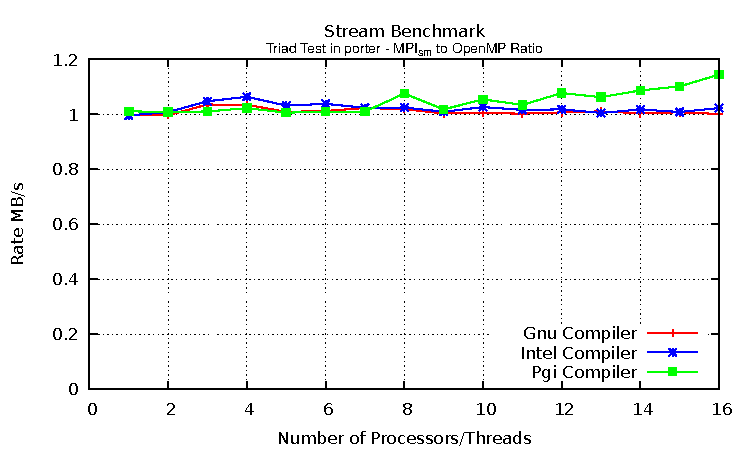
\includegraphics[width=0.95\linewidth]{Plots/streamBenchmark/porter-TriadRatio.pdf}
      \caption{Execution time}
      \label{fig:TriadRatio}
    \end{subfigure}
\caption{Triad test.}
\label{fig:TriadTestt}
\end{figure}






\begin{comment}


Two identical versions of the stream benchmarks one using  and 
 were created and it 
 results are compared below for several systems. 
 
 
 However, the arrays 



 capabilities of the 

an MPI$_{sm}$ version of the program was developed and used to compare its performance to that obtained using its 



OpenMP versions of the STREAM benchmark program has been used to measure the evolution of the sustainable memory bandwidth of shared memory system as more threads are included in the test. 




What is STREAM?
The STREAM benchmark is a simple synthetic benchmark program that measures sustainable memory bandwidth (in MB/s) and the corresponding computation rate for simple vector kernels. 

Why should I care?

Computer cpus are getting faster much more quickly than computer memory systems. 

As this progresses, 

As an extreme example, several current high-end machines run simple arithmetic kernels for out-of-cache operands at 4-5 percent of their rated peak speeds --- that means that they are spending 95-96 percent of their time idle and waiting for cache misses to be satisfied.

The STREAM benchmark is specifically designed to work with datasets much larger than the available cache on any given system, so that the results are (presumably) more indicative of the performance of very large, vector style applications.

If you want more words, I have written a paper on STREAM: Sustainable Memory Bandwidth in Current High Performance Computers

A somewhat broader look on the issue, see my paper: Memory Bandwidth and Machine Balance in Current High Performance Computers. STREAM is also a useful component of models for scaling of homogeneous throughput workloads (like the SPEC CPU "rate" benchmarks). 

Examples of models based on STREAM measurements that do a pretty good job of estimating SPECfp rate2000 scaling are included in several presentations.

\end{comment}

